\documentclass[11pt, a4paper]{article}
%\usepackage{proj1}
\usepackage{natbib}
\usepackage{fancyhdr}  
\usepackage{subcaption}
\usepackage{caption}
\usepackage{graphicx}
\usepackage{numprint}
\usepackage{multirow}
\linespread{1.25} 
\setlength{\parindent}{0cm}
\graphicspath{{Images/}}
\usepackage{hyperref}
\usepackage{amsmath}
\usepackage{amsfonts}
\usepackage{amssymb}
\usepackage{amsthm}
\usepackage{mathtools}
\usepackage{commath}
\usepackage{bbm}

%\usepackage[sc,osf]{mathpazo}
\usepackage{subcaption}
\usepackage[a4paper, top=1in, left=1.0in, right=1.0in, bottom=1in, includehead, includefoot]{geometry} %Usually have top as 1in

\usepackage{listings}
\usepackage{color} %red, green, blue, yellow, cyan, magenta, black, white
\definecolor{mygreen}{RGB}{28,172,0} % color values Red, Green, Blue
\definecolor{mylilas}{RGB}{170,55,241}


\hypersetup{colorlinks,linkcolor={black},citecolor={blue},urlcolor={black}}
\usepackage{color}
\urlstyle{same}


\theoremstyle{definition}
\newtheorem{definition}{Definition}[section]

\newcommand{\adja}{q_a}
\newcommand{\adjb}{q_b}
\newcommand{\adjaB}{q_{a,\partial \Omega}}
\newcommand{\adjbB}{q_{b,\partial \Omega}}
\newcommand{\adjB}{q_{\partial \Omega}}
\newcommand{\Adja}{\mathbf{p}}
\newcommand{\Adjb}{q}
\newcommand{\adj}{q}
\newcommand{\Adjc}{{q}_{\partial \Omega}}
\newcommand{\ra}{\rho_a}
\newcommand{\rb}{\rho_b}
\newcommand{\w}{\mathbf{w}}
\newcommand{\f}{\mathbf{f}}
\newcommand{\ve}{\mathbf{v}}
\newcommand{\n}{\mathbf{n}}
\newcommand{\h}{\mathbf{h}}
\newcommand{\K}{\mathbf{K}}
\newcommand{\hr}{\widehat \rho}
\newcommand{\jf}{\mathbf j}

%	\begin{figure}[h]
%		\centering
%		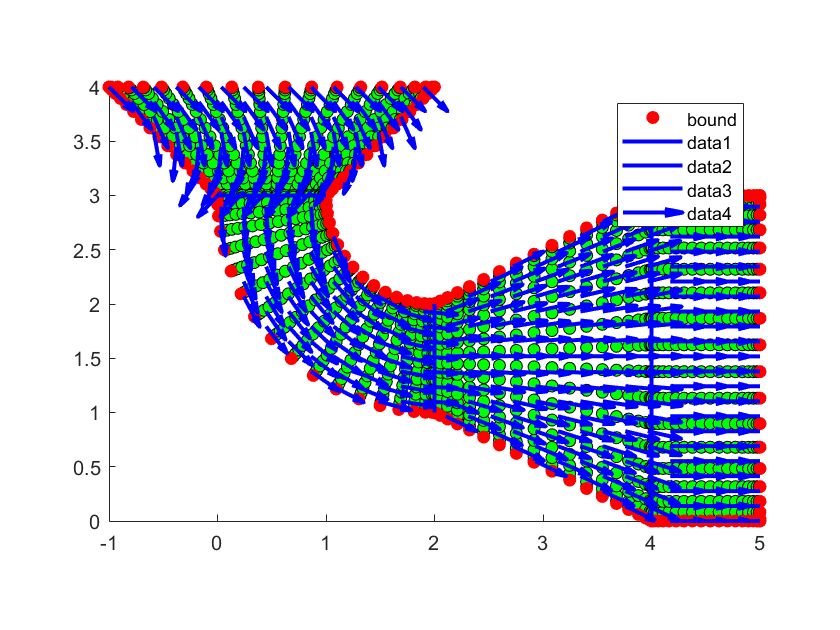
\includegraphics[scale=0.35]{F1.png}
%		\caption{Forward $\rho$ for $a = 0.01$} 
%		\label{F1}
%	\end{figure}

\begin{document}
\section*{18/02/2021}	
	
	
	\section*{OPC Periodic}
    We attempt to compute an OCP in a periodic box. We choose $n = 30$ and $N = 50$. As before, the target has a gravitational strength of $c = 0.1$, while the OCP equation has $c = 0.01$, $\kappa = -3.5$ and $\beta = 10^{-3}$. We chose the domain to be 'the wrong way round' - needs to be redone to account for flip of plotting domain.
    The result is $J_{FW} = 0.3243$ and $J_{Opt} = 0.0522$. The result can be seen in Figure \ref{F1}. Note that the code for flipping the plotting domain for the flux is not written yet.
	
		\begin{figure}[h]
			\centering
			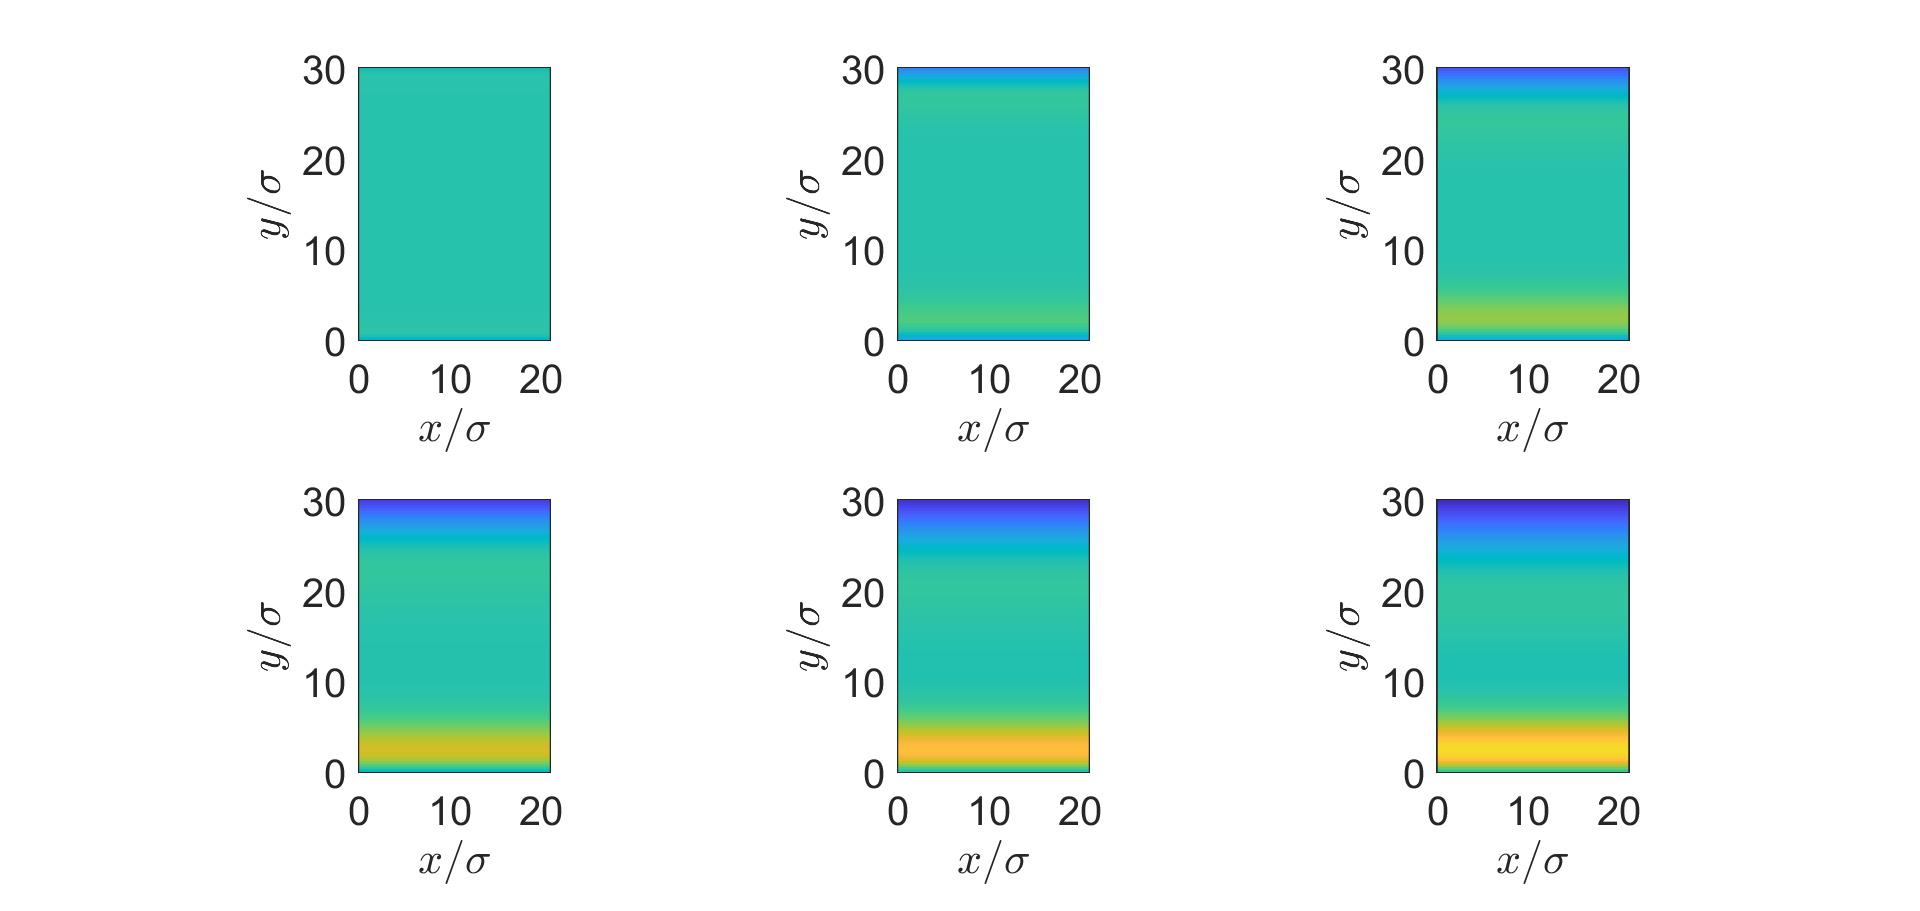
\includegraphics[scale=0.35]{rho1.png}
			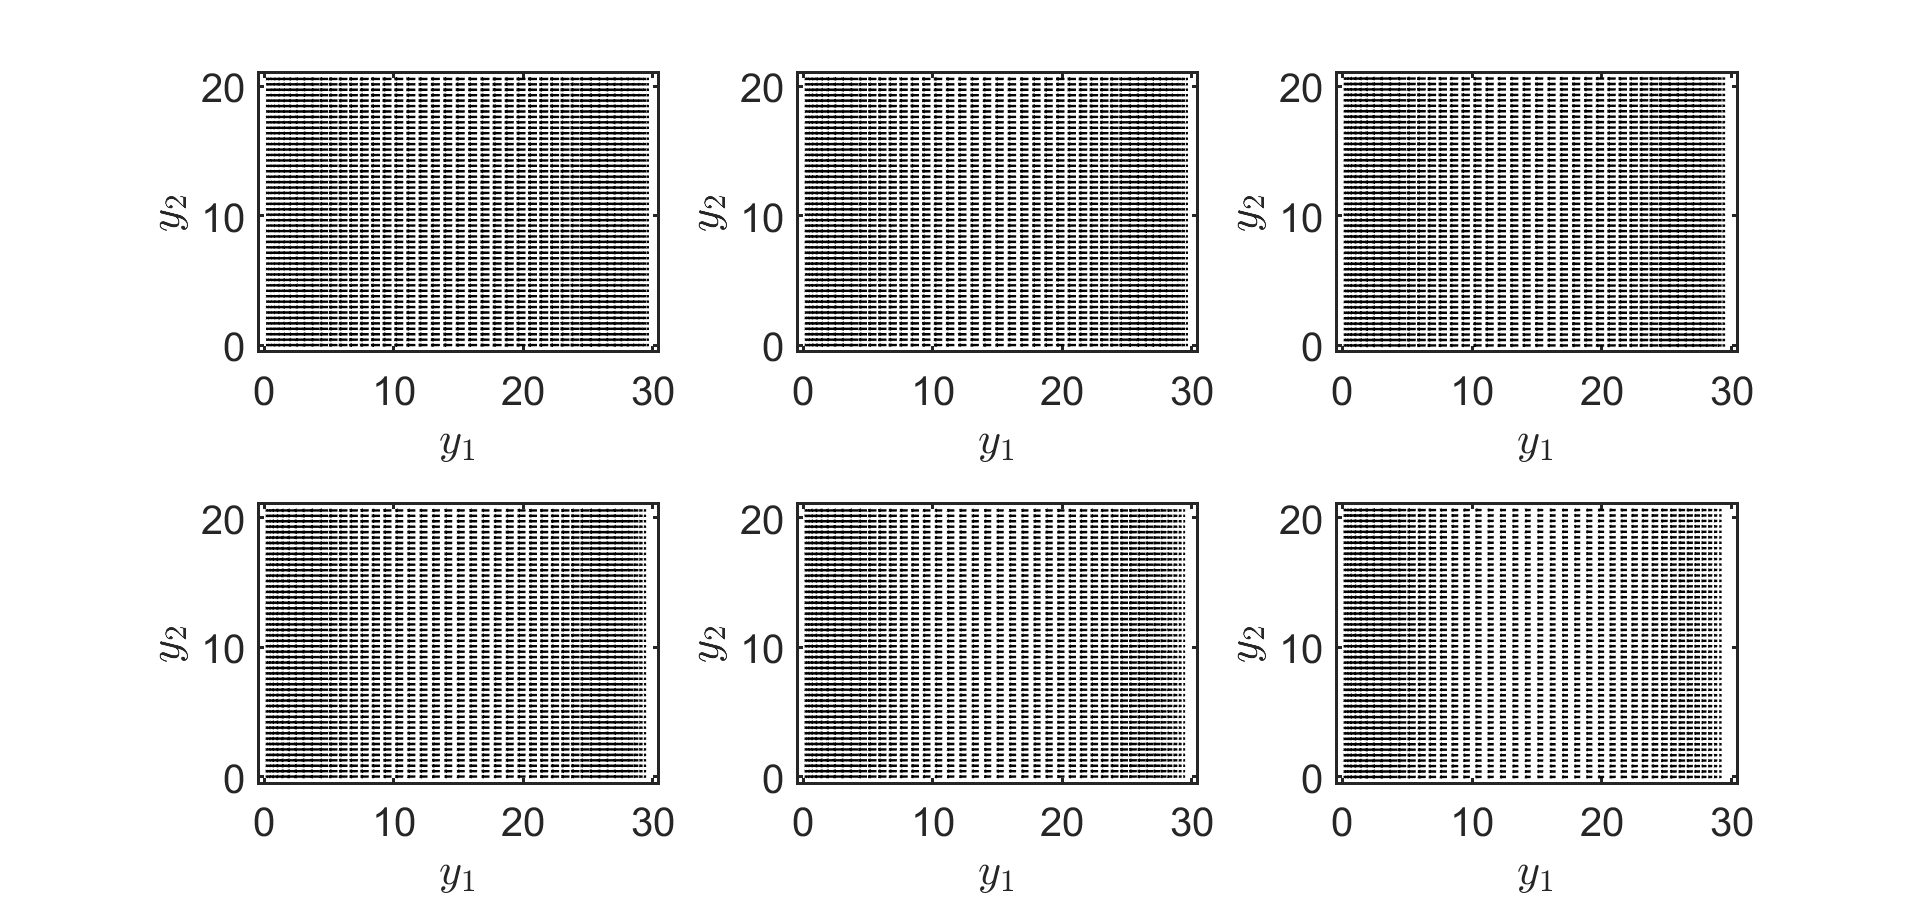
\includegraphics[scale=0.35]{control1.png}
			\caption{Optimal $\rho$ and optimal control} 
			\label{F1}
		\end{figure}
	
	
	\section{Multishape/ Wedge Issue}
	There is an issue with the multishape involving a wedge. This is mainly important when we have interactions on. Figures \ref{F2} and \ref{F2a} demonstrate the issues. Is it possible that imposing $V_{Ext} = c y_2$ causes issues with the wedge and the boundaries between wedge and other shapes? It seems fine when plotting $V_{ext}$, see Figure \ref{F2b}.
	I can produce negative cost functionals with this... 

	\begin{figure}[h]
		\centering
		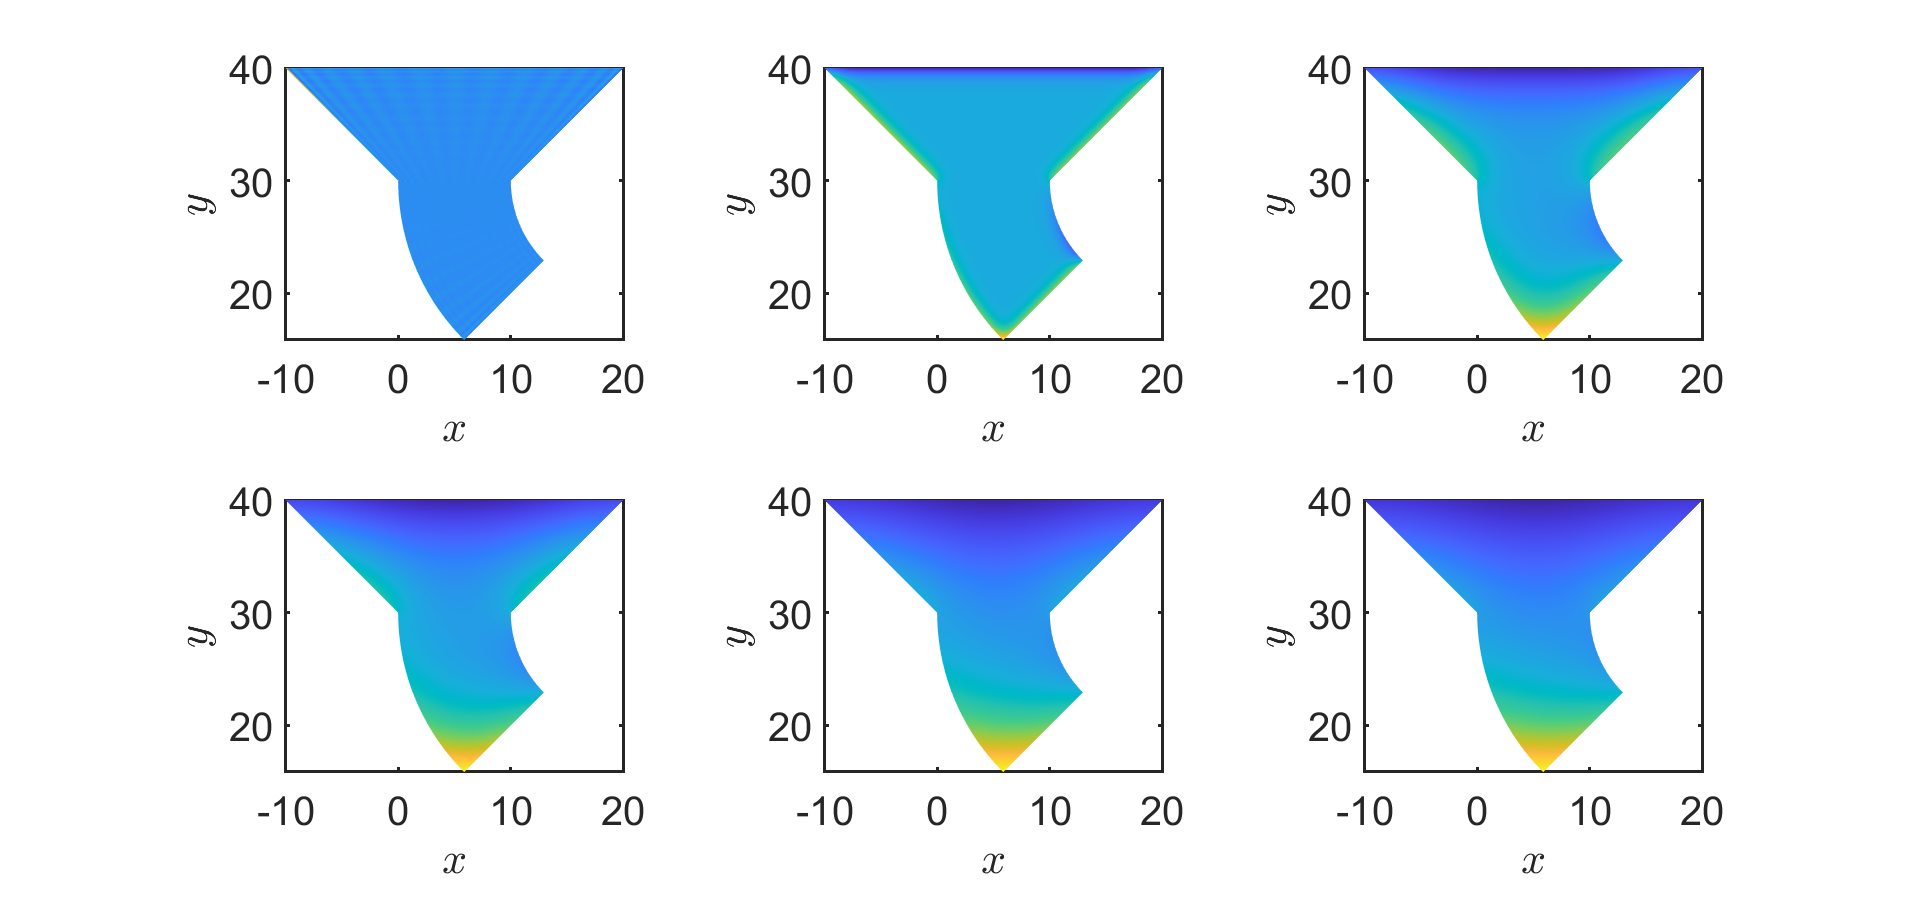
\includegraphics[scale=0.35]{demo2.png}
		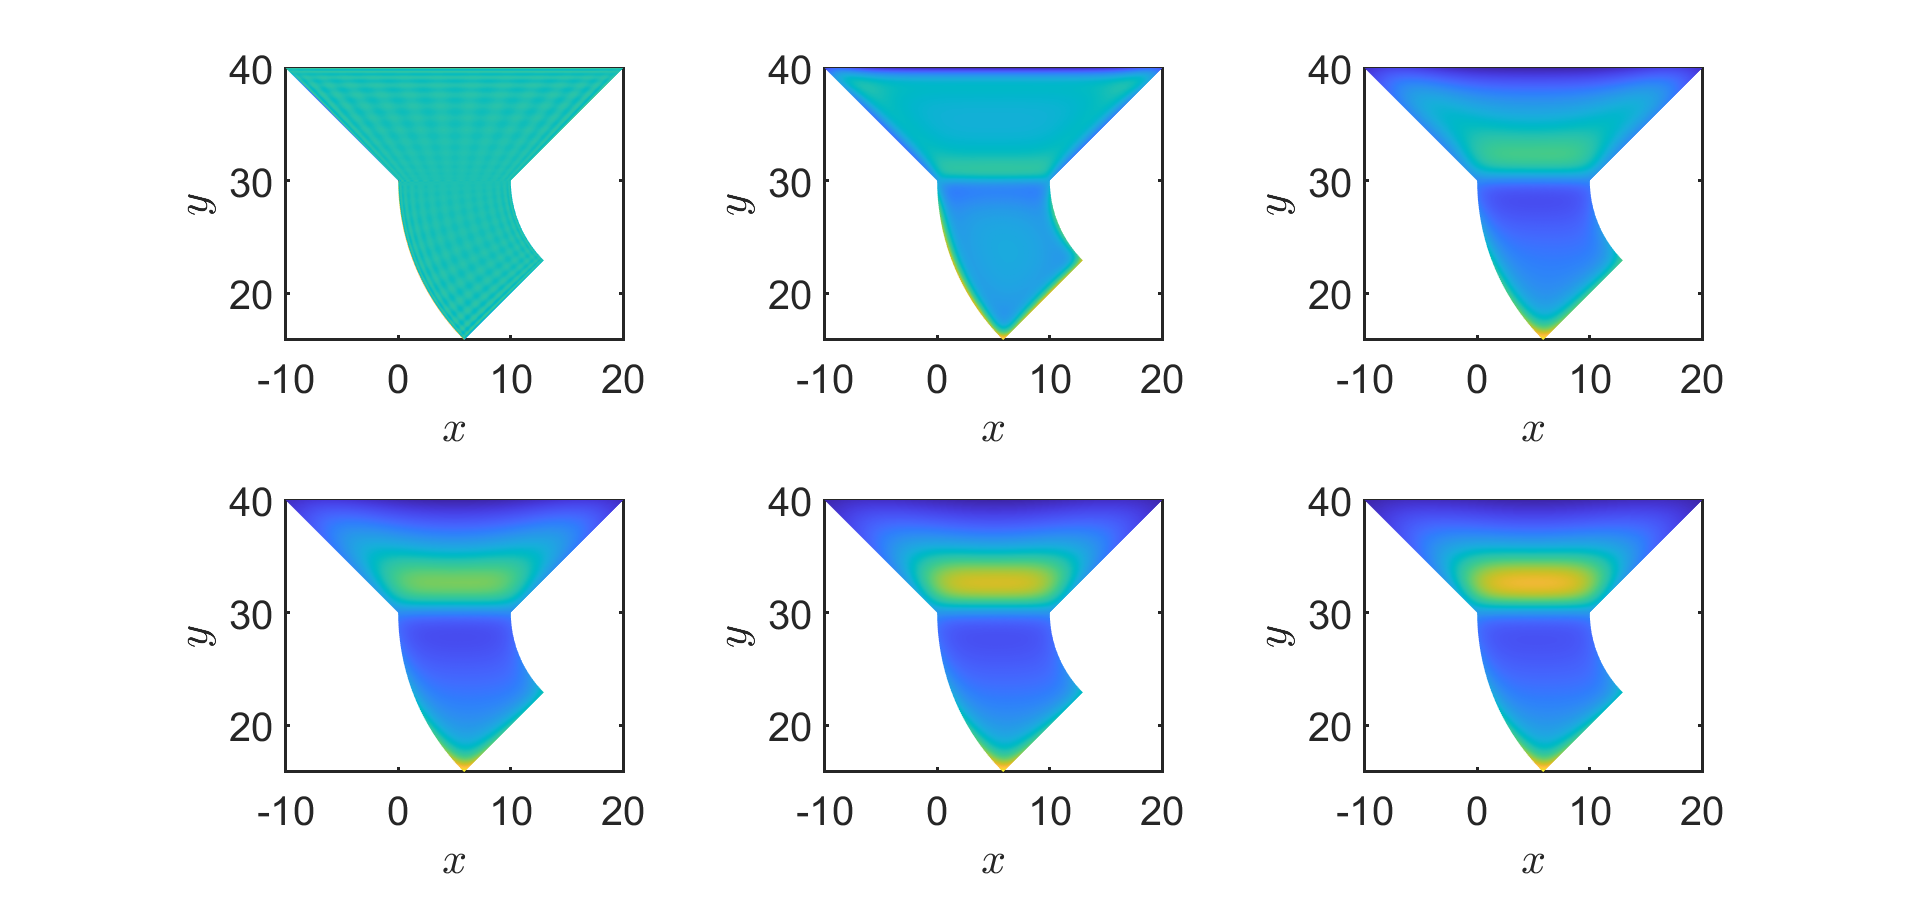
\includegraphics[scale=0.35]{demo1.png}
		\caption{Issue with wedge 1} 
		\label{F2}
	\end{figure}
		\begin{figure}[h]
		\centering
		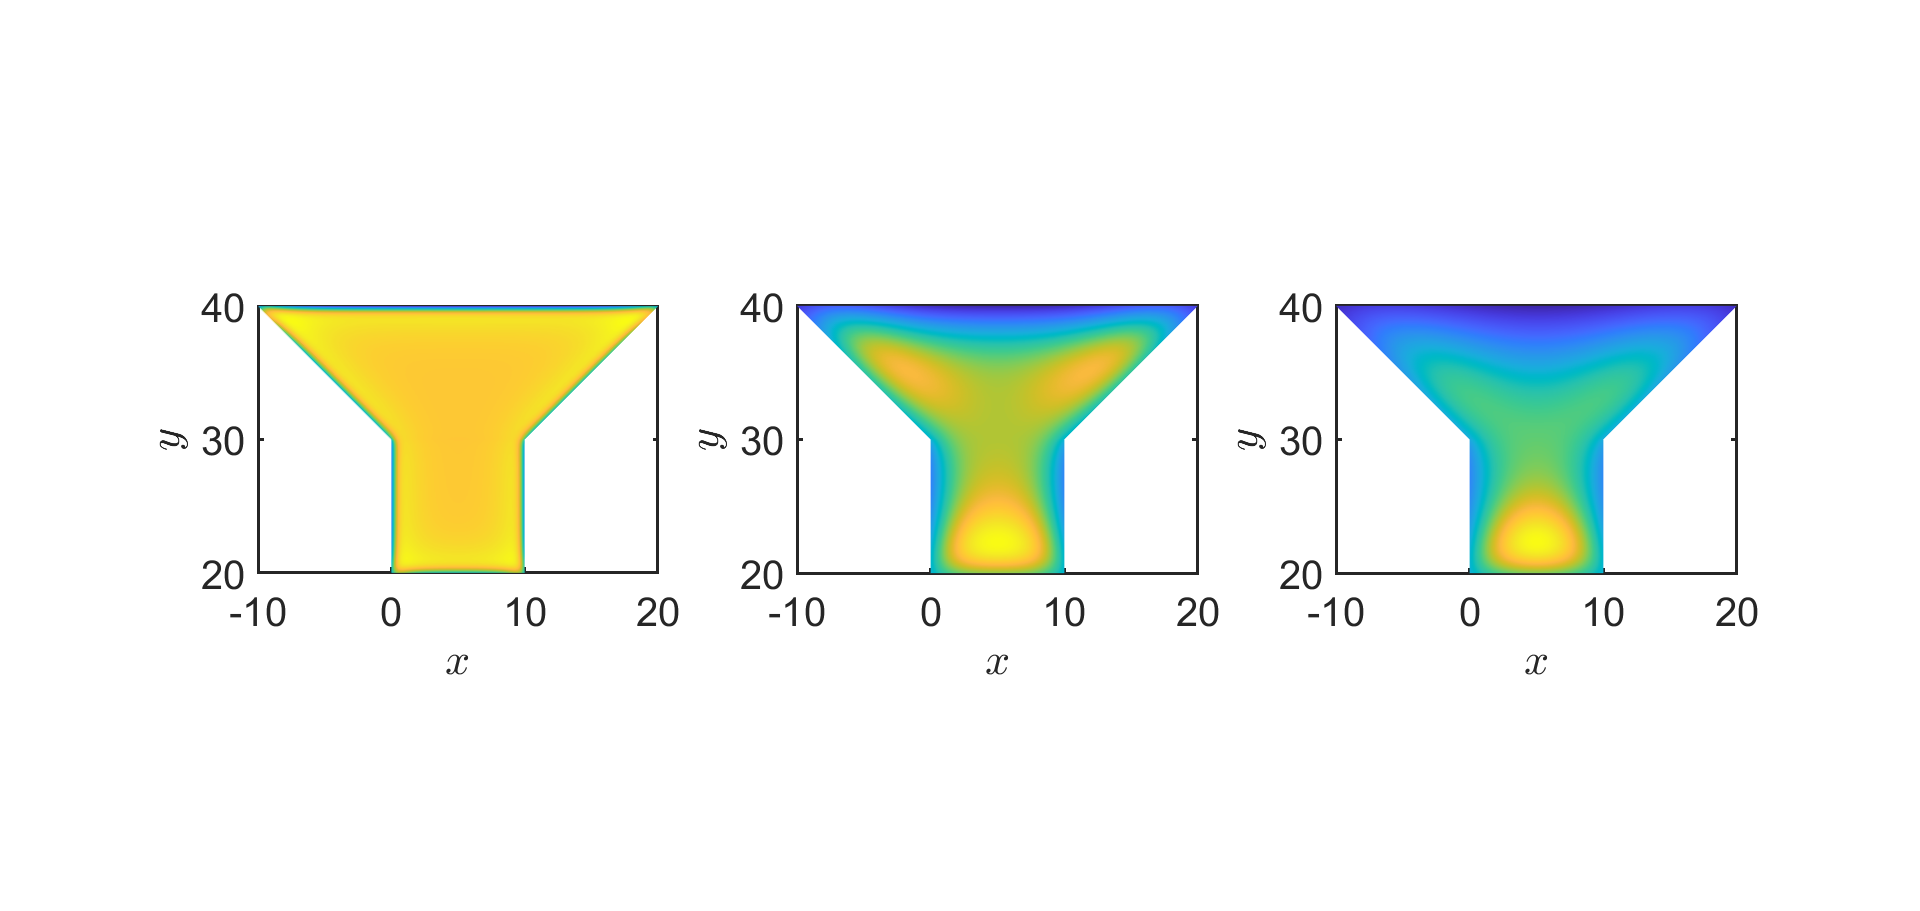
\includegraphics[scale=0.35]{demo3.png}
		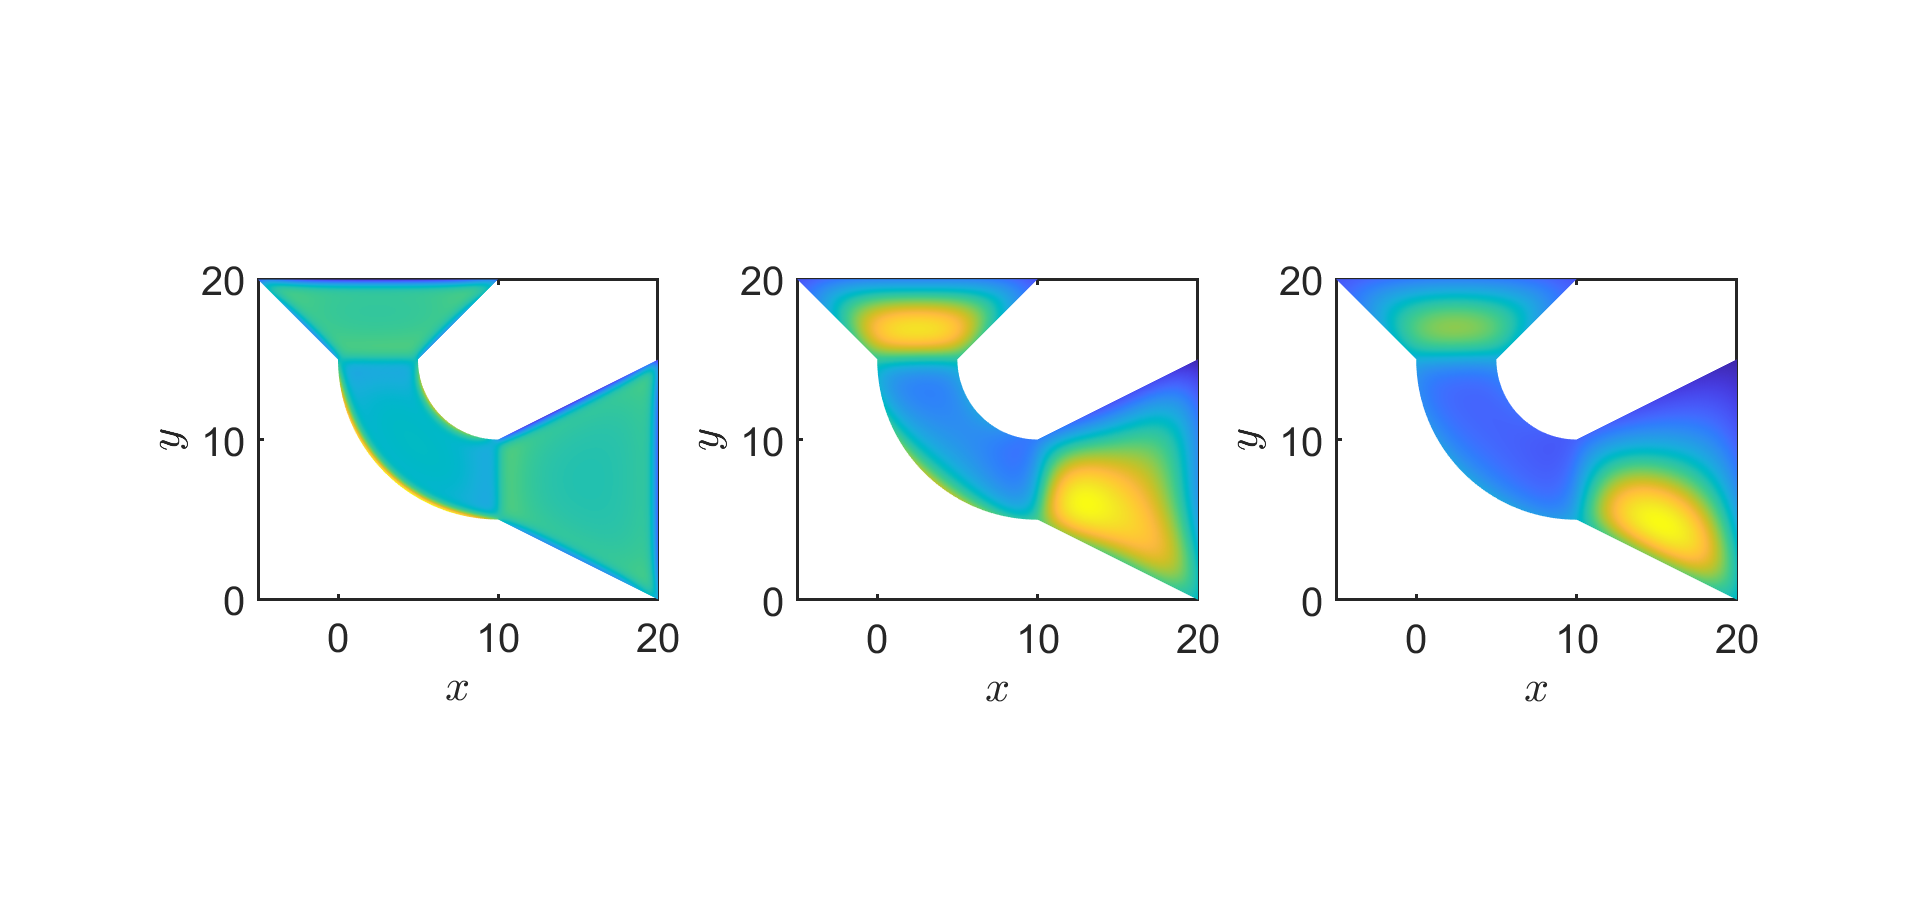
\includegraphics[scale=0.35]{demo4.png}
		\caption{Issue with wedge 2} 
		\label{F2a}
	\end{figure}
	\begin{figure}[h]
		\centering
		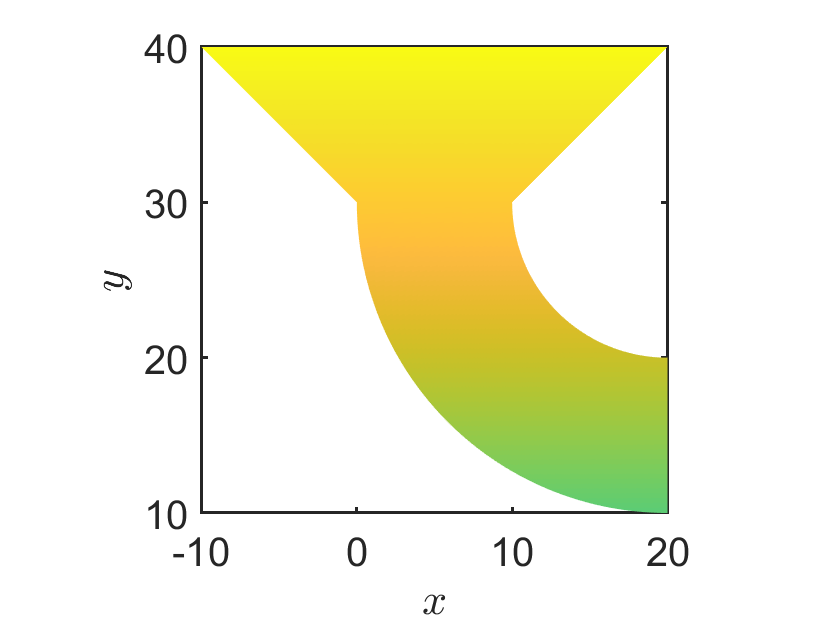
\includegraphics[scale=0.35]{demo5.png}
		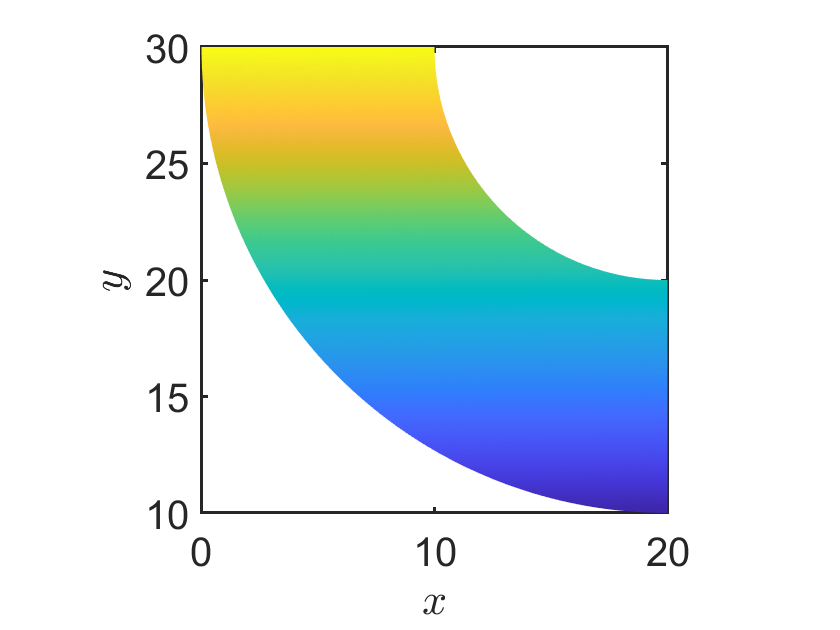
\includegraphics[scale=0.35]{demo6.png}
		\caption{Issue with wedge, $V_{ext}$} 
		\label{F2b}
	\end{figure}

	\section{Two more issues and questions}
	1. Mistake in calculating the cost functional in the code - I think it doesn't affect the results but should still be changed -- in paper code too? See Figure \ref{F3}.\\
	2. 3D to 2D averaging still doesn't work.\\
	3. Papers on sedimentation $f$?
	
	\begin{figure}[h]
		\centering
		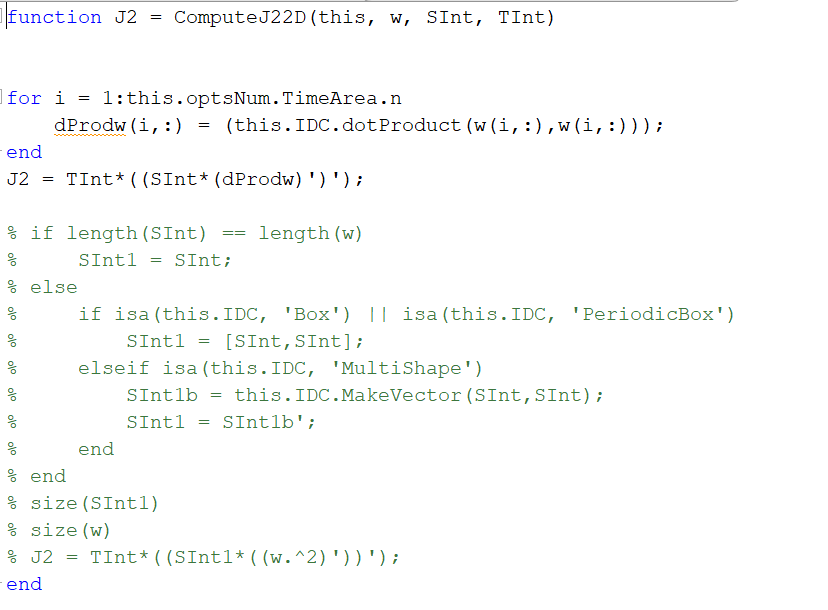
\includegraphics[scale=0.7]{error.png}
		\caption{Error in J2} 
		\label{F3}
	\end{figure}
	
	
	\section{Periodic Boundary Conditions for a General Flux}

We consider the advection diffusion equation with periodic boundary conditions and a corresponding OCP:
\begin{align*}
	&\min \frac{1}{2}|| \rho - \hr||^2 + \frac{\beta}{2}||\w||^2\\
	&\text{subject to:}\\
	&\frac{\partial \rho}{\partial t} = \nabla \cdot \left(\nabla \rho - \rho \w\right) = \nabla \cdot \jf\\
	& \rho|_{\partial \Omega_l} = \rho|_{\partial \Omega_r}\\
	& \rho|_{\partial \Omega_t} = \rho|_{\partial \Omega_b}\\
	& - \jf \cdot \n |_{\partial \Omega_l}= - \jf \cdot \n|_{\partial \Omega_r}
\end{align*}
such that $\partial\Omega_l \cup \partial\Omega_r = \partial \Omega$ and the abbreviations corresponding to left and right respectively. Top and bottom boundaries are omitted, since, as shown in the previous section, they follow analogously and are independent of the results on the left and right boundary.
The relevant part of the Lagrangian is then:
\begin{align*}
	\mathcal{L} &= ... -\int_0^T \int_\Omega \left(\frac{\partial \rho}{\partial t} - \nabla \cdot \jf\right)q dr dt - \int_0^T \int_{\partial \Omega_l} \left(- \rho q_1 - \jf \cdot \n q_2 \right) dr  + \int_{\partial \Omega_r} \left(\rho q_1 +  \jf \cdot \n q_2  \right)  dr .
\end{align*}
Integrating by parts, and omitting terms in $\Omega$, gives:
\begin{align*}
	\mathcal{L} &= ... - \int_0^T \int_{\partial \Omega}- q \jf  \cdot \n - \mathbf{k}(\rho, q) \cdot \n  dr dt - \int_0^T \int_{\partial \Omega_l} \left(- \rho q_1 - \jf \cdot \n q_2 \right)   dr  + \int_{\partial \Omega_r} \left(\rho q_1 + \jf \cdot \n q_2 \right)   dr, 
\end{align*}
where $\mathbf{k}$ are any terms arising from integrating by parts a second time.
We now need to take the Frech\'et derivative of $\jf$ with respect to $\rho$. This cannot be done in general, because $\jf$ does not only depend on $\rho$ but also on $\mathbf r$. In each case we need to calculate:
\begin{align*}
	\jf'(h) := \jf (\rho + h) - \jf (\rho).
\end{align*}
Similarly, we need to take the derivative of $\mathbf k$ and denote it by $\mathbf{k}'$.
Denoting this Frech\'et derivative by $\jf'(h)$ we can write out further terms as follows:
\begin{align*}
	\mathcal{L}_\rho &= ... - \int_0^T \int_{\partial \Omega}- q \jf'(h)   \cdot \n - \mathbf{k}' \cdot \n dr dt - \int_0^T \int_{\partial \Omega_l} \left(- h q_1 - \jf'(h)  \cdot \n q_2 \right)   dr  + \int_{\partial \Omega_r} \left(h q_1 + \jf'(h)  \cdot \n q_2 \right)   dr dt. 
\end{align*}
When writing out the terms explicitly we pay attention to the fact that $\n|_{\partial \Omega_l} = - \n|_{\partial \Omega_r}$ and $\n|_{\partial \Omega_t} = - \n|_{\partial \Omega_b}$.
\begin{align*}
	\mathcal{L}_\rho &= ... - \int_0^T \int_{\partial \Omega_l} \left(- h q_1 - q \jf'(h)   \cdot \n  - \mathbf{k}' \cdot \n- \jf'(h)  \cdot \n q_2 \right)   dr  \\
	&+ \int_{\partial \Omega_r} \left(h q_1 + q \jf'(h)   \cdot \n + \mathbf{k}' \cdot \n+ \jf'(h)  \cdot \n q_2 \right)   dr dt .
\end{align*}
In order to proceed further, we need to split up $\jf'(h)$ into two parts as follows:
\begin{align*}
	\jf'(h) = \jf'_1(h) + h \jf'_2,
\end{align*}
so that $\jf'_1$ is applied to $h$, since it depends on $\mathbf{r}$ as well (e.g. the Frech\'et derivative of $\nabla \rho$) and $\jf'_2$ is applied to another function and multiplied by $h$ (e.g. h $\frac{\partial }{\partial n}$ applied to $q$). We do the same for $\mathbf k'$.
We then have:
\begin{align*}
	\mathcal{L}_\rho &= ... - \int_0^T \int_{\partial \Omega_l} \left(- h q_1 - q \jf_1'(h)   \cdot \n - \mathbf{k}_1' \cdot \n - \jf_1'(h)  \cdot \n q_2  - h \jf'_2 q \cdot \n - h \mathbf{k}_2' \cdot \n-  h \jf'_2 q_2 \cdot \n \right)   dr  \\
	&+ \int_{\partial \Omega_r} \left( h q_1 + q \jf_1'(h)   \cdot \n +\mathbf{k}_1' \cdot \n+ \jf_1'(h)  \cdot \n q_2 + h\mathbf{k}_2' \cdot \n + h \jf'_2 q \cdot \n +  h \jf'_2 q_2 \cdot \n \right)   dr dt.
\end{align*}
Now considering all terms such that $h \neq 0$ on each boundary separately, we get:
\begin{align*}
	&\int_0^T \int_{\partial \Omega_l} \left(- h q_1  - h \jf'_2 q \cdot \n - h\mathbf{k}_2' \cdot \n-  h \jf'_2 q_2 \cdot \n \right)   dr  dt =0 \\
	&\int_0^T \int_{\partial \Omega_r} \left( h q_1  + h \jf'_2 q \cdot \n + h\mathbf{k}_2' \cdot \n + h \jf'_2 q_2 \cdot \n \right)   dr  dt =0 ,
\end{align*}
and so, as in the previous sections, we have:
\begin{align*}
	q_1 &= -  \jf'_2 q \cdot \n - h\mathbf{k}_2' \cdot \n - \jf'_2 q_2 \cdot \n |_{\partial \Omega_l} \\
	q_1 &= -  \jf'_2 q \cdot \n -  h\mathbf{k}_2' \cdot \n -\jf'_2 q_2 \cdot \n |_{\partial \Omega_r}, 
\end{align*}
which gives:
\begin{align*}
	\jf'_2 q \cdot \n +  \mathbf{k}_2' \cdot \n + \jf'_2 q_2 \cdot \n |_{\partial \Omega_l} =  \jf'_2 q \cdot \n + \mathbf{k}_2' \cdot \n +  \jf'_2 q_2 \cdot \n |_{\partial \Omega_r}.
\end{align*}
But since $q_2|_{\partial \Omega_l} = q_2|_{\partial \Omega_r}$, we can conclude that:
\begin{align*}
	\jf'_2 q \cdot \n + \mathbf{k}_2' \cdot \n  |_{\partial \Omega_l} =  \jf'_2 q \cdot \n + \mathbf{k}_2' \cdot \n  |_{\partial \Omega_r}.
\end{align*}
Considering now $\jf'_1 \neq 0$, we get:
\begin{align*}
	\int_0^T \int_{\partial \Omega_l} \left(- q \jf_1'(h)   \cdot \n  - \mathbf{k}_1' \cdot \n - \jf_1'(h)  \cdot \n q_2  \right)   dr  + \int_{\partial \Omega_r} \left(q \jf_1'(h)   \cdot \n + \mathbf{k}_1' \cdot \n + \jf_1'(h)  \cdot \n q_2  \right)   dr dt = 0 .
\end{align*}
Again, since $q_2|_{\partial \Omega_l} = q_2|_{\partial \Omega_r}$, we have that:
\begin{align*}
	\int_0^T \int_{\partial \Omega_l}  q \jf_1'(h)   \cdot \n  +\mathbf{k}_1' \cdot \n   dr dt = \int_0^T \int_{\partial \Omega_r} q \jf_1'(h)   \cdot \n  +  \mathbf{k}_1' \cdot \n  dr dt .
\end{align*}
Writing this in terms of the integrand only can be done for each specific case of $\jf_1'$ and $\mathbf{k}_1'$. 
\\
\\
An example: Let $\jf = \nabla \rho - \rho \w$ as above. Then we have that $\jf_1'(h) = \nabla h$ and $\jf_2' = \w $. From integration by parts we will get that $\mathbf k = - \rho \nabla q$, so $\mathbf k_1' = 0$ and $\mathbf k_2' = -  \nabla q$.
We get that:
\begin{align*}
	&q\w  \cdot \n  - \nabla q \cdot \n |_{\partial \Omega_l} = q\w  \cdot \n  - \nabla q \cdot \n |_{\partial \Omega_r},
\end{align*}
and
\begin{align*}
	\int_0^T \int_{\partial \Omega_l}  q \nabla h   \cdot \n    dr dt = \int_0^T \int_{\partial \Omega_r} q \nabla h  \cdot \n    dr dt,
\end{align*}
and so 
\begin{align*}
	q |_{\partial \Omega_l} = q|_{\partial \Omega_r},
\end{align*}
as required.	
	
	
	
	
	
	
	
	
\end{document}